%! Author = maxwe
%! Date = 12.01.23

% Preamble
\documentclass{scrartcl}

% Packages
\usepackage{amsmath}
\usepackage{graphicx}
\usepackage{biblatex}
\usepackage{tabularray}
\UseTblrLibrary{booktabs}

\usepackage{symbols}
\usepackage{hyperref}

% Document
\begin{document}

    \title{Documentation for the pyroll-thermal-2d Plugin}
    \author{Max Weiner}
    \date{\today}

    \maketitle


    \section{Model Description}\label{sec:model-description}

    \begin{figure}
        \centering
        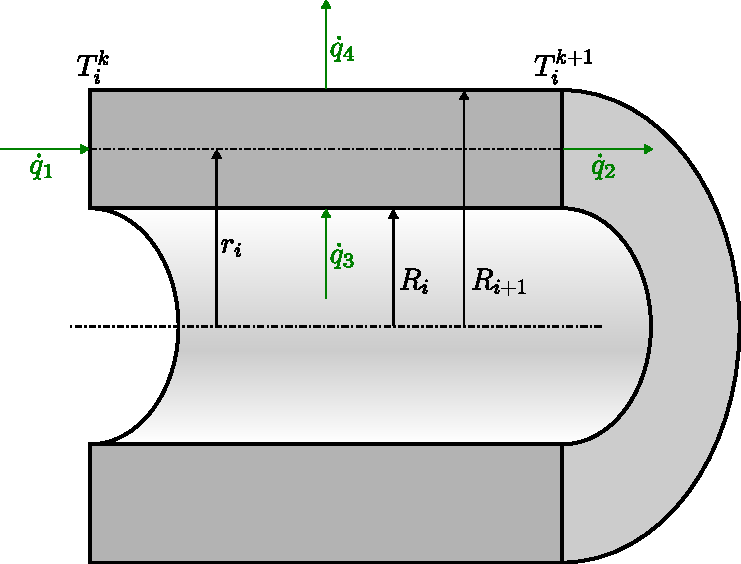
\includegraphics[scale=0.8]{img/heat_flow}
        \caption{Heat Flows on a Disk Element Ring}
        \label{fig:heat_flow}
    \end{figure}

    \subsection{Heat Flow Balance}

    see \autoref{fig:heat_flow}, $\RIndex$ index of layer in radial direction, $\XIndex$ index of disk element in x-direction

    \begin{equation}
        0 = \HeatFlow_1 - \HeatFlow_2 - \HeatFlow_3 + \HeatFlow_4 + \HeatSource
        \label{eq:heat_flow_balance}
    \end{equation}

    heat flow contributions

    \begin{equation}
        \HeatFlow_1 = \Density \ThermalCapacity \VolumeFlow \Temperature_{\RIndex}^{\XIndex}
        \label{eq:heat_flow_1}
    \end{equation}

    \begin{equation}
        \HeatFlow_2 = \Density \ThermalCapacity \VolumeFlow \Temperature_{\RIndex}^{\XIndex+1}
        \label{eq:heat_flow_2}
    \end{equation}

    \begin{equation}
        \HeatFlow_3 = -\ThermalConductivity \frac{\Temperature_{\RIndex+1}^{\XIndex}-\Temperature_{\RIndex}^{\XIndex}}{\RadiusWidth} \times 2 \pi \left( \Radius_\RIndex + \frac{\RadiusWidth}{2} \right) \XWidth
        \label{eq:heat_flow_3}
    \end{equation}

    \begin{equation}
        \HeatFlow_4 = -\ThermalConductivity \frac{\Temperature_{\RIndex}^{\XIndex}-\Temperature_{\RIndex-1}^{\XIndex}}{\RadiusWidth} \times 2 \pi \left( \Radius_\RIndex - \frac{\RadiusWidth}{2} \right) \XWidth
        \label{eq:heat_flow_4}
    \end{equation}

    \begin{equation}
        \HeatSource = \HeatSourceEfficiency \frac{\FlowStress}{\FormingEfficiency} \Strain \VolumeFlow
        \label{eq:heat_source}
    \end{equation}

    at surface different $\HeatFlow_3$, with surface temperature $\SurfaceTemperature$

    \begin{equation}
        \HeatFlow_3 = \left[ -\HeatTransferCoefficient \left( \EnvironmentTemperature - \SurfaceTemperature \right) - \RadiationCoefficient\RelativeRadiationCoefficient\left( \EnvironmentTemperature^4 - \SurfaceTemperature^4 \right) \right]
        \times 2 \pi \left( \Radius_\RIndex + \frac{\RadiusWidth}{2} \right) \XWidth
        \label{eq:heat_flow_3_surface}
    \end{equation}

    surface temperature estimation as stationary state between environment and outer layer, numerical solution

    \begin{equation}
        2 \ThermalConductivity \frac{\SurfaceTemperature - \Temperature_\RIndexMax^\XIndex}{\RadiusWidth} = \HeatTransferCoefficient \left( \EnvironmentTemperature - \SurfaceTemperature \right) + \RadiationCoefficient\RelativeRadiationCoefficient\left( \EnvironmentTemperature^4 - \SurfaceTemperature^4 \right)
        \label{eq:surface_temperature}
    \end{equation}

    \subsection{Temperature Increment Functions}

    for core layer $\HeatFlow_4 = 0$

    \begin{equation}
        \TemperatureIncrement_0 = \frac{1}{\Density\ThermalCapacity\VolumeFlow_0} \left[ \pi \ThermalConductivity \XWidth \left( \Temperature_1^\XIndex - \Temperature_0^\XIndex \right) + \HeatSource{}_0 \right]
        \label{eq:increment_core}
    \end{equation}

    for intermediate layers with \autoref{eq:heat_flow_3}

    \begin{equation}
        \TemperatureIncrement_\RIndex = \frac{1}{\Density\ThermalCapacity\VolumeFlow_\RIndex}
        \left[
            \frac{2 \pi \ThermalConductivity \XWidth}{\RadiusWidth} \left[
                \left( \Temperature_{\RIndex+1}^\XIndex - \Temperature_\RIndex^\XIndex \right)
                \left( \Radius_\RIndex + \frac{\RadiusWidth}{2} \right)
                -\left( \Temperature_{\RIndex}^\XIndex - \Temperature_{\RIndex-1}^\XIndex \right)
                \left( \Radius_\RIndex - \frac{\RadiusWidth}{2} \right)
                \right]
            + \HeatSource{}_\RIndex
            \right]
        \label{eq:increment_layer}
    \end{equation}

    for surface layer with \autoref{eq:heat_flow_3_surface}

    \begin{equation}
        \TemperatureIncrement_\RIndexMax = \frac{1}{\Density\ThermalCapacity\VolumeFlow_\RIndex}
        \left[
        2 \pi \XWidth \left[
        \left[ \HeatTransferCoefficient \left( \EnvironmentTemperature - \SurfaceTemperature \right) + \RadiationCoefficient\RelativeRadiationCoefficient\left( \EnvironmentTemperature^4 - \SurfaceTemperature^4 \right) \right]
        \left( \Radius_\RIndex + \frac{\RadiusWidth}{2} \right)
        -\ThermalConductivity \frac{\Temperature_{\RIndex}^\XIndex - \Temperature_{\RIndex-1}^\XIndex}{\RadiusWidth}
        \left( \Radius_\RIndex - \frac{\RadiusWidth}{2} \right)
        \right]
        + \HeatSource{}_{\RIndex}
        \right]
        \label{eq:increment_surface}
    \end{equation}


    \section{Plugin Usage}\label{sec:plugin-usage}

    \addsec{Symbols}

\begin{longtblr}[
    label= none,
    entry = none
]{ll}
    \toprule
    Symbol & Description \\
    \midrule
    
    ${{s["code"]}}$ & {{s["descr"]}}\\
    
    \bottomrule
\end{longtblr}

    \printbibliography


\end{document}